\documentclass[border=20pt]{standalone}
\renewcommand\familydefault{\sfdefault} % Default family: serif 
%\usepackage[usenames,dvipsnames]{xcolor}
\usepackage[x11names]{xcolor}
\usepackage{tikz}
\usepackage{soulutf8}
\usetikzlibrary{arrows,fit,positioning,shapes,calc}

%\definecolor{WIRE}{HTML}{002FA7} % Klein Blue
\usepackage[normalem]{ulem}

\tikzstyle{every entity} = []
\tikzstyle{every weak entity} = []
\tikzstyle{every attribute} = []
\tikzstyle{every relationship} = []
\tikzstyle{every link} = []
\tikzstyle{every isa} = []

\tikzstyle{link} = [>=triangle 60, draw, thick, every link]

\tikzstyle{total} = [link, double, double distance=3pt]

\tikzstyle{entity} = [rectangle, draw, black, very thick,
minimum width=6em, minimum height=3em,
every entity]

\tikzstyle{weak entity} = [entity, double, double distance=2pt,
every weak entity]

\tikzstyle{attribute} = [ellipse, draw, black, very thick,
minimum width=5em, minimum height=2em,
every attribute]

%\tikzstyle{key attribute} = [attribute, font=\bfseries]

\tikzstyle{multi attribute} = [attribute, double, double distance=2pt]

\tikzstyle{derived attribute} = [attribute, dashed]

%\tikzstyle{discriminator} = [attribute, font=\itshape]

\tikzstyle{relationship} = [diamond, draw, black, very thick,
minimum width=2em, aspect=1,
every relationship]

\tikzstyle{ident relationship} = [relationship, double, double distance=2pt]

\tikzstyle{isa} = [isosceles triangle, isosceles triangle apex angle=60,
shape border rotate=-90,
draw, black, very thick, minimum size=3em,
every isa]

% for text un key attributes
\newcommand{\key}[1]{\underline{#1}}
\newcommand{\pkey}[1]{\dashuline{#1}}

% for text in discriminator attributes
\def\discriminator{\bgroup 
	\ifdim\ULdepth=\maxdimen  % Set depth based on font, if not set already
	\settodepth\ULdepth{(j}\advance\ULdepth.4pt\fi
	\markoverwith{\kern.15em
		\vtop{\kern\ULdepth \hrule width .3em}%
		\kern.15em}\ULon}

%%


\definecolor{MediumPurple1}{rgb}{0.58, 0.44, 0.86}
\definecolor{Chartreuse2}{rgb}{0.5, 1.0, 0.0}
\tikzset{every entity/.style={draw=orange, fill=orange!20}}
\tikzset{every attribute/.style={draw=MediumPurple1, fill=MediumPurple1!20}}
\tikzset{every relationship/.style={draw=Chartreuse2, fill=Chartreuse2!20}}

%% Variable for participation constraint
\newcommand{\cM}{\mathrm{M}}
\newcommand{\cN}{\mathrm{N}}
\newcommand{\cO}{\mathrm{O}}
\newcommand{\cP}{\mathrm{P}}

\begin{document}


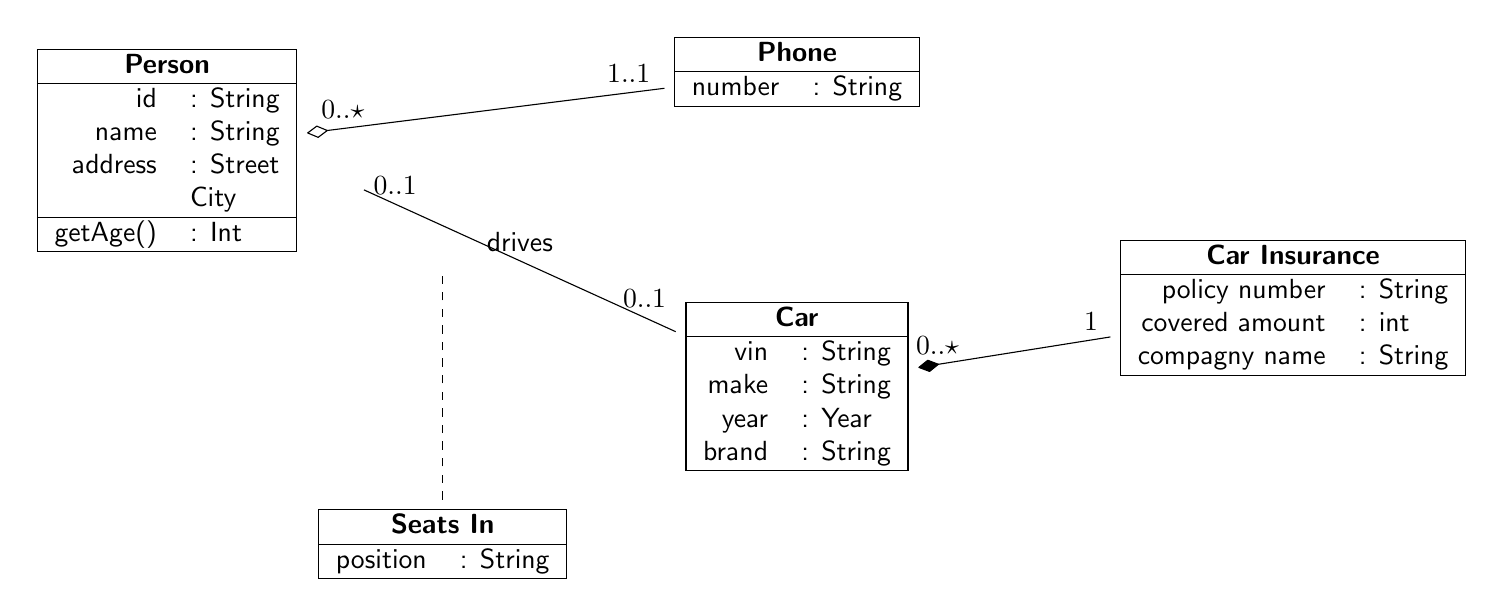
\begin{tikzpicture}
	\node (person) at (0,0){\begin{tabular}{| r l |}
			\hline
			\multicolumn{2}{| c |}{\textbf{Person}} \\
			\hline
			id       & : String                \\
			name     & : String                \\
			address  & : Street                \\
			         & City                    \\
			\hline
			getAge() & : Int                   \\
			\hline
		\end{tabular}
	};
	\node (phone) at (8, 1){\begin{tabular}{| r l |}
			\hline
			\multicolumn{2}{| c |}{\textbf{Phone}} \\
			\hline
			number & : String                 \\
			\hline
		\end{tabular}
	};
	\draw[open diamond-] (person) -- node[above, pos=0.1]{$0..\star$} node[above, pos=0.9]{$1..1$} (phone);
	\node (car) at (8, -3){\begin{tabular}{| r l |}
			\hline
			\multicolumn{2}{| c |}{\textbf{Car}} \\
			\hline
			vin   & : String                \\
			make  & : String                \\
			year  & : Year                  \\
			brand & : String                \\
			\hline
		\end{tabular}
	};
	\draw[-] ($(person)+(2.5,-0.5)$) -- node[above, pos=0.1]{$0..1$} node[above, pos=0.5]{drives} node[above, pos=0.9]{$0..1$} (car);
	%\draw[-] (person) -- node[below, pos=0.1]{$0..1$} node[below, pos=0.9]{$0..4$} ($(car)+(-2.5, 0.5)$);
	\node (seat) at (3.5, -5){\begin{tabular}{| r l |}
			\hline
			\multicolumn{2}{| c |}{\textbf{Seats In}} \\
			\hline
			position & : String                  \\
			\hline
		\end{tabular}
	};
	\draw[dashed] (seat) -- (3.5, -1.6);

	\node (insu) at (14.3, -2){\begin{tabular}{| r l |}
			\hline
			\multicolumn{2}{| c |}{\textbf{Car Insurance}} \\
			\hline
			policy number  & : String                 \\
			covered amount & : int                    \\
			compagny name  & : String                 \\
			\hline
		\end{tabular}
	};

	\draw[diamond -] (car) -- node[above, pos=0.1]{$0..\star$} node[above, pos=0.9]{$1$} (insu);
\end{tikzpicture}
\end{document}